\documentclass{article}
\usepackage[utf8]{inputenc}
\usepackage[]{amsmath}
\usepackage{amsthm,amssymb}
\usepackage{enumerate}% http://ctan.org/pkg/enumerate
\usepackage{hyperref}
\usepackage{tikz}
\usepackage{ mathrsfs}
\usepackage[margin=0.5in]{geometry}

\usepackage{tikz}
\usepackage{pgfplots}

% no indents pls
\setlength\parindent{0pt}


%%% defs for theorem environments
\renewcommand{\qedsymbol}{\rule{0.7em}{0.7em}} % black box for QED
\newtheorem*{thm}{Theorem}
\newtheorem{lem}{Lemma}
% defining style for Cases
\newtheoremstyle{casestyle}{\topsep}{1pt}{}{0pt}{\itshape}{.}{5pt plus 1pt minus 1pt}{}
\theoremstyle{casestyle}
\newtheorem{case}{Case}
% smallcaps-ing "Proof" header
\let\oldproofname=\proofname
\renewcommand{\proofname}{\rm\sc{\oldproofname}}

\begin{document}

\section *{Problem 1}
Our data structure is an augmented balanced BST over the indexes (from $1$ to $n$). That is to say, for a node $N$, all nodes with smaller indexes are in the left subtree and all nodes with larger indexes are in the right subtree. For a node at index $i$ (which we will denote $N_i$, we augment it with a few pieces of information:\\

$1$) $p_i$ - the price at index $i$\\
$2$) $P_i$ - the maximum single-sell profit within the range of $i$ and all its children. \\
$3$) $p_{i, smallest}$ and $p_{i, largest}$ - the smallest and largest prices, respectively, within the range of $i$ and all its children. \\

$P_i$, $p_{i, smallest}$, $p_{i, largest}$ are calculated by simply looking at its two immediate children $N_l$ (left child) and $N_r$ (right child) as follows: \\
$P_i = max(P_l,\ P_r,\ p_{r, largest} - p_{l, smallest},\ p_i - p_{l, smallest},\ p_{r, largest} - p_i) $\\
$p_{i, smallest} = min(p_i, p_{l, smallest}, p_{r, smallest})$\\
$p_{i, largest} = max(p_i, p_{l, largest}, p_{r, largest})$\\
If node at $i$ has no children, $P_i = 0$, $p_{i, smallest} = p_{i, largest} = p_i$\\

\begin{proof} Of Correctness\\
  For any given node $N_i$, we will prove that $P_i$, $p_{i, smallest}$, and $p_{i, largest}$ are of the correct values. Our base case: if $N_i$ has no children, then we have only $p_i$ to work with. Therefore, $P_i$ must be $0$ because we must sell immediately after we buy, and $p_i$ is both the largest and the smallest price.\\

  By induction, assume the left and right subtrees of $N_i$ have the correct values. We will now prove that $N_i$'s values are correct. Observe that all the indexes in the left subtree of $N_i$ are smaller than $i$, and all the indexes in the right subtree are greater than $i$. Therefore, $N_i$ acts as a kind of "bridge" between the two subtrees. Let $N_{buy}$ and $N_{sell}$ be the two nodes responsible for $P_i$ in our given range. We see there can be only five possibilities for where these two nodes can be located:\\

  1) $N_{buy}$ and $N_{sell}$ are both in the left subtree of $N_i$. This value already exists in the left child of $N_i$ as $P_l$.\\
  2) $N_{buy}$ and $N_{sell}$ are both in the right subtree of $N_i$. This value already exits in the right child of $N_i$ as $P_r$.\\
  3) $N_{buy}$ is in the left subtree and $N_{sell}$ is in the right subtree. Note the positions cannot be switched, because you must buy before you sell. In this case, $P_i$ must equal the difference between the smallest price in the left subtree and the largest price in the right subtree. Any other combination will yield a smaller price difference, and therefore a smaller profit. This value is calculated as $p_{r, largest} - p_{l, smallest}$.\\
  4) $N_{buy}$ is in the left subtree of $N_i$ and $N_{sell} = N_i$. $P_i$ must then equal the difference between $p_i$ and the smallest price in the left subtree of $N_i$, calculated as: $p_i - p_{l, smallest}. $\\
  5) $N_{buy} = N_i$ and $N_{sell}$ is in the right subtree of $N_i$. $P_i$ must then equal the difference between the largest price in the right subtree of $N_i$ and $p_i$. \\

  Because these are the only five possibilities, $P_i$ must equal the largest of these values. And it takes constant time for calculate because the necessary values can be accessed in either $N_i$ or in its immediate children.\\

  The proof of correctness of $p_{i,smallest}$ and $p_{i, largest}$ is almost trivial. The smallest price of a tree rooted at $N_i$ must either be $p_i$ or the smallest price in either the left or right subtree. The same logic applies for the largest price. The takes constant time to evaluate. \\
\end{proof}

Having proven that augmentation works and be calculated in constant time per node, we describe and prove the correctness and runtime of the following operations:\\

\textbf{ds.mssp()}\\
The maximum single-sell profit for the current list is simply $P_{root}$, because $P_{root}$ is defined as the value of the maximum single-sell profit for $N_{root}$ and its all children. This takes $O(1)$ time to obtain because the value has already been computed in the root node.

\textbf{ds.insert(i, p)} \\
Insert $N_i$ by traversing the BST with $i$. Initialize the values in $N_i$. Traverse back up, up to and including the root, updating the stored values at each parent. The will preserve the correctness of our tree, because the stored values at each node depends only on its children and itself. Nodes not on this path need not update.\\

Calculating the new value of a node takes $O(1)$ time as shown above. There are $log(n)$ nodes on the path back to the root, because our BST is balanced. Searching a BST takes $O(log(n))$ time also, so our final runtime is $O(log(n))$\\

\textbf{ds.update(i, p)}\\
Find $N_i$ by traversing the BST with $i$. Update the price in $N_i$. Update the stored values in $N_i$, as well as the stored values in every ancestor of $N_i$ up to and including the root. As with ds.insert(i, p), this preserves the correctness of the tree, and takes $O(log(n))$, since the length of the path back to the root is bounded by the height of our balanced BST. (Finding a node in a balanced BST also takes $O(log(n))$). \\

\textbf{ds.remove(i)}\\
Remove $N_i$ as you would any node from a balanced BST. However, remember the the parent of $N_i$'s in-order successor as you delete. Update the stored values in this parent, as well all the nodes from this parent back to (an including) the root. If $N_i$ is a leaf node, update the stored values in $N_i$ all of $N_i$'s parents. This preserves correctness, because when $N_i$ is removed, its in-order successor is hoisted up to replace it. Therefore, the in-order successor's ancestors must all be updated. The hoisted in-order successor will automatically be updated this way because $N_i$ must have been an ancestor of the successor's previous position.\\

Removing a node from a balanced BSD takes $O(log(n))$ time. Updating each node takes constant time, and the number of updates is bounded by the height of the tree $(log(n))$. This gives a final runtime of $O(log(n))$.\\

\newpage

\section *{Problem 2}
Our algorithm uses the split($T$, $k$) and join($T_1$, $k$, $T_2$) algorithms presented in lecture. We will define our removal range to be $(k_1, k_2]$. That is to say, we will remove all the elements between $k_1$ and $k_2$, not including $k_1$ but including $k_2$.\\

First, call split($T$, $k_1$) to produce $T_{left}$ (tree of smaller values) and $T_{rest}$ (tree of larger values). Then, call split($T_{rest}$, $k_2$) to produce $T_{remove}$ (tree of smaller values) and $T_{right}$ (tree of larger values). Delete all the nodes in $T_{remove}$. Next, find and remove the largest key $x$ from $T_{left}$ and then call join($T_{left}$, $x$, $T_{right}$) and set the resulting tree equal to $T$. \\

\begin{proof} Of Correctness.\\
  By definition of split($T$, $k$), $T_{left}$ will contain all keys in $T$ less then or equal too $k_1$. After the second split, $T_{right}$ will contain all the keys in $T$ strictly greater than $k_2$. This means that $T_{remove}$ must contain all the keys in $T$ greater than $k_1$ and less than or equal to $k_2$. This is exactly the subset of keys we want to delete.\\

  We must rejoin the remaining two trees to produce our new $T$ after this range excision. In order to call join on $T_{left}$ and $T_{right}$, we must find a "bridging" key greater than all the keys in $T_{left}$ and less than all the keys in $T_{right}$. The largest key in $T_{left}$ satisfies this condition, as long as it is removed from $T_{left}$ (so it can be greater than all the keys in $T_{left}$. Therefore, we have all the necessary arguments to call join and produce our resulting $T$.\\

\end{proof}

\begin{proof} Of Runtime.\\
  By definition, split($T$, $k$) runs in time $O(log(n))$ and join($T_1$, $k$, $T_2$) runs in time equal to the difference between the heights of $T_1$ and $T_2$. because $T_1$ and $T_2$ come from the same balanced binary tree, this height difference is bounded by $log(n)$. Deleting all nodes in $T_{remove}$ takes $O(z)$ time, because every node in $T_{remove}$ is in the range to be excised, and removing/freeing a node takes $O(1)$. Finally, finding the largest key in the BST $T_{left}$, by definition, takes time $O(log(n))$. Our algorithm does is call split twice and join once, resulting a final runtime of $O(3log(n) + log(n) + z) = O(log(n) + z)$.\\

\end{proof}

\newpage

\section *{Problem 3}
\begin{enumerate}[i]
\item 
  Create a balanced BST for the indexes from $1$ to $n$. Every node $N$ stores the sum of all the nodes in the left subtree of $N$ (including $N$, so leaf nodes initialize themselves to their own value).  The tree must be initialized from bottom up, so that every node only needs to look at its immediate left child to calculate its "left sum". Because there are $n$ nodes, and calculating the left sum for every node takes $O(1)$ time, the total initialization time is $O(n)$.\\

  For the following descriptions and proofs, we define "left parent" to mean the parent of a right child node. "Right parent" means the parent of a left child node. A node can have either a left parent or a right parent, but not both.\\

  \textbf{ds.increment(i, x)}\\
  Find the correct node by performing a binary search for $i$. Add $x$ to the value of this node, as well as to all of its ancestors that are right parents themselves. \\

  This will preserve the correctness of the left sums, because the only nodes that need to be updated are right parents. Note that this is true because any ancestor of $i$ that is a right parent must be greater than $i$ and therefore have node $i$ in its left subtree. Performing a binary search for $i$ takes $O(log(n))$ time. The number of ancestors we need to look at is bounded by the height of the tree, which is $O(log(n))$, and is our final runtime for this method.\\

  \textbf{ds.cumulativeFrequency(i)}\\
  Find the correct node by performing a binary search for $i$. Keep a global sum to update - starting at the value of node $i$. Then, for each ancestor of node $i$ that is a left parent, add the left sum to our global sum, and return the global sum as the cumulative frequency.\\

  As one traverses up the tree, due to BST properties, every new left parent we come across must have a lower index then any node we have already added to the cumulative frequency. Therefore, no node can ever be added to our calculated sum twice. We prove that every node from $1$ to $i$ is counted. By contradiction; assume there is some index $k$ that is in the range but is somehow not counted in the cumulative frequency. Because $k < i$, $k$ must be a node to the left of $i$ in the BST, and they must share some ancestor $A$. Therefore, $k$ must be in the left subtree of $A$ (or be $A$) and $i$ must be in the right subtree of $A$ (or be $A$). However, this means that $A$ must be a left parent on the path from $i$ to back to the root, because $A < i$ and our path back to the root, by definition, counts all ancestors of $i$ where $ A < i$. The left subtree of $A$, and therefore $k$, must have therefore been counted in the cumulative frequency of $i$.\\

  Performing a binary search for $i$ takes $O(log(n))$ time. The number of ancestors we need to look at is bounded by the height of the tree, which is also $O(log(n))$, and is our final runtime for this method.

\item
  See code

\item
  Our implementation uses a single, $1$-indexed array from $1$ to $n$. Unlike our described algorithm in part $i$, we do not need to perform binary search, but instead we can simply index into the array in constant time. However, our array is implicitly structured as a tree. In order to find the index of the next left parent on the path from node $x$ back to the root, we calculate $x - (x \& -x)$. And in order to find the index of the next right parent on the path from node $x$ back to the root, we calculate $x + (x \& -x)$. We stop when the calculated index becomes $0$. \\

  Our tree is no longer necessarily a balanced BST. The nodes are stored in in-order sequence, such than an in-order traversal of the BST will produce the indexes $1$ to $n$, in order. The entire left spine of our BST are consecutive powers of two starting from $2^0$ at the bottom left). Only the left side of our BST is therefore guaranteed to be complete. The right subtree will only ever been complete if $n = 2^k - 1$ for some $k$. Specifically, if $2^m$ is the smallest power of two larger than $n$, the right subtree will be missing $2^m - 1 - n$ nodes from its right side. So our right subtree would still structured as if it was complete, but with a number of its rightmost nodes removed. If the removal of any of these nodes creates an "orphan" left subtree, there must be some "adoption" node in the right subtree (including the root) that now has no right child. Therefore we simply connect the root of the orphan tree as the right child of the adoption node - preserving BST.\\

  Note that despite this heavily lopsided tree, the overall height of the tree is still $O(log(n)$, because $n$ will never be more than a constant factor of two away from the next largest power of two.\\

  The reason our implicit tree is structured this way is for our bitwise operations to work. For a given index $x$, $x \& -x$ gives us the smallest bit in $x$ that is set (to $1$). For example, for the number $6$, represented in binary $110$, $6 \& -6$ is $010$ in binary. If one structures their tree the way we did above, you see that:\\

  1) The next left parent on the path from node $x$ to the root can be calculated by removing the smallest bit in $x$, which which can be done through subtraction: $x - (x \& -x)$. We can detect when $x$ has no more left parents, because the left spine of our BST are all powers of two, so subtracting away the leftmost bit gives $0$, an invalid index. \\
  2) The next right parent the path from non-root node $x$ to the root can be calculated by adding the smallest bit in $x$. Hence: $x + (x \& -x)$. We can detect when $x$ has no more right parents, because our addition creates a number greater than $n$. \\

  Knowing these tricks, we are able to implement a Fenwick tree following the approach described in part $i$.\\

  \newpage

  \section *{Problem 4}
  \begin{enumerate}[i]
  \item Encoding skiplist as multiway tree. Let each node in a skiplist be of level $1$ to $k$, where level $i$ indicates that the node has $i$ forward pointers, from $1$ to $i$. We begin with a skiplist $L$ with $n$ nodes and a highest level of $k_{\max}$ (this is the level of the node in $L$ with the highest level). To encode $L$ as a multiway tree $T$, we start at level $k_{\max}$; all of the nodes with a level of $k_{\max}$ are keys in the root node of $T$. We then continue down the levels in the same way: each node of level $k$ in $L$ will translate to a key in a node of depth $k_{\max}-k$ in $T$. The nodes on this level $k$ that are not separated by any nodes of level $>k$ are clustered together in the same node $j$ in $T$ as keys. The parent of $j$ is the node of depth $k_{\max}-k-1$ in $T$ such that the range of keys in $j$ falls into the ``key space'' of that node, as explained in lecture 5. The root node has no parent. We repeat this until level $1$, the bottom of $L$ and the encoding is complete. If no appropriate parent in the level immediately above can be found, keep traversing up levels until a parent can be found. This can be shown in the diagram, in which the node with ``4'' starts out as level 1 nodes, but is a direct child of the root node, since there is no other node of level 2 between the ``3'' node and ``5'' node \\\\
    Encoding a multiway tree as a skip list. Let $k_{\max}-1$ be the maximum depth of the tree $T$ that will be encoded to list $L$. We begin by creating a simple linked list of all the items in sorted 
    order. We then start from depth $k_{\max}-2$ in $T$ and link together (with forward pointers)/elevate (to level $2$) nodes in $L$ that correspond to keys in nodes of depth $k_{\max}-2$  in $T$. We repeat this process, linking together nodes in $L$ and elevating them to level $i$ for every depth $k_{\max}-i$ in $T$ until depth $0$. Note that ``elevation'' occurs as a side effect of the linkage and is not an independent process in itself.
    \\\\
    Note that while this creates an isometry between the skiplist and multiway tree, it is possible that converting a skiplist to multiway tree and back does not result in the original skiplist. This is due to the fact there may be levels of the skiplist with the exact same nodes and thus no meaningful corresponding node in the tree i.e.\ there are more skiplists than valid multiway trees. This can be illustrated in the following diagram, where a skiplist is encoded to a multiway tree, which is then encoded back to the skiplist.

    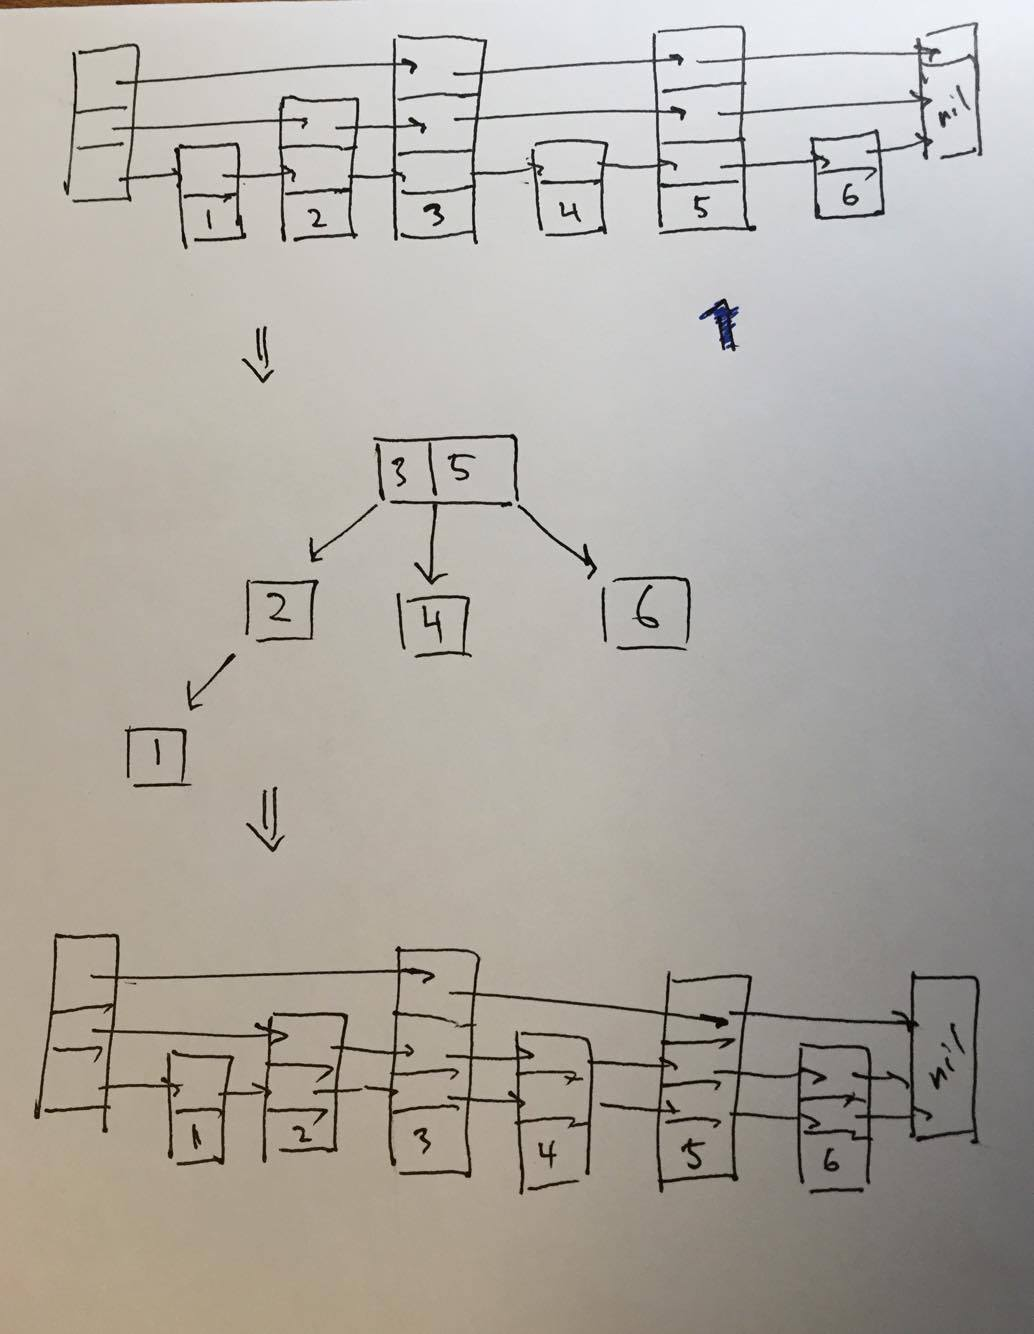
\includegraphics[scale=.3]{4i}

  \item We will walk through the B-tree rules and translate as follows: \begin{enumerate}
    \item The root node has between $1$ and $2b-1$ keys $\rightarrow$ $L$ can only have $1$, $2$, or $3$ nodes linked together at the highest level $k_{\max}$.
    \item All non-root nodes have between $b-1$ and $2b-1$ keys $\rightarrow$ At every subsequent level $k_i$, there can be $1$, $2$, or $3$ nodes linked together of level $i$ between nodes of any level greater than $i$ or the two ends of the list.
    \item All leaf nodes are stored at the same depth and all root-null paths through the tree pass through the same number of nodes $\rightarrow$ At every level $i$ such that $i > 1$, there must be at least one node of level $i-1$ between every node of a level $i$ or higher or the two ends of the list.
    \item The B-tree is a BST and has sorted nodes $\rightarrow$ The nodes on level $i$ between nodes of level $i$ or higher or the two ends of the list must be sorted, have values less than the next node of level $i+1$ (unless the next node is an end node or we are at the top of the tree) and have values greater than the previous node of level $i+1$ (same conditions apply as before).
    \end{enumerate}

  \item Due to the isometry between the 1-2-3 List $L$ and 2-3-4 Tree $T$, we can perform a similar algorithm to a B-tree lookup. We first traverse the nodes on the top level in $L$ sequentially until we find the key or get to a node on that level just before the key (we would have to do a lookahead to ensure this). If the key is not found, descend one level on the node where the search stopped and recursively explore that lower level in the same way, descending as needed, until the node containing the key is found. At the lowest level, no descending can be done, so we must traverse until we reach the key or overshoot and conclude that the key does not exist. This emulates a B-Tree lookup, since descending one level and following that pointer is equivalent to following a child connection in the B-Tree lookup. Thus, due to their isometry, the lookup time on a 1-2-3 List will be asymptotically identical to that of a 2-3-4 Tree lookup: $O(\log n)$ per lecture.

  \item Algorithm: In order to insert element $e$. We first perform a lookup to find the location of the node, $p$ right before the element to be inserted. This is done via the same lookup mechanism as described in the previous part, with the minor modification that when we overshoot on the lowest level, we keep track of the node right before. During this traversal, we also keep track of the nodes at which a descent to a lower level occurred. \\\\ Since $p$ is guaranteed to have level 1 based on 1-2-3 List properties (property (c)), we can insert element $e$ as a node right after $p$ on the same level (level 1). We then go back and ensure that this does not violate property (b) that there can be no more than $3$ nodes of level $1$ between nodes of any level $>1$. We can check this since we kept track of the nodes at which a descent occurred. Thus, we can start from node containing the descent to level $1$, $d$ and count the number of nodes of level $1$ between $d$ and the next node with a level $>1$. If this number is $1$, $2$ or $3$, then nothing needs to be done. Otherwise, there are $4$ nodes and we elevate the third node from the left by inserting it on the level above (level 2 in this case) between $d$ and the node that $d$ points to on that level. We now perform this check on the next level to ensure that there are not $4$ nodes on level 2 and continue in the same fashion (checking against the previous descent node and elevating up) until we reach the top level $k_{\max}$. If there end up being $4$ nodes connected on level $k_{\max}$, then we elevate the third node as before (with the node connecting only to the beginning and end, ``nil'' nodes of the list on that level) and the new top level of the list becomes $k_{\max}+1$.
    \\\\ Correctness: Since insertion is always after the position that the element would have been at on the bottom level, the property listed in (d) of 1-2-3 Lists is not violated by the initial insertion. In the case of an elevation of a node to a higher level, property (d) is still not violated since it is inserted into the the list of higher level in sorted order. Since elevating the third node in clusters of $4$ nodes of the same level produces two and one nodes separated by the new node, we do not violate property (a) or (b). Since we are only inserting elements and the elevation still preserves at least one node of the original level in between nodes of the new level, we do not violate property (c). Thus, after insertion, our list is still a 1-2-3 list.
    \\\\ Runtime: The initial lookup takes $O(\log n)$ time as shown in the previous part. Each elevation takes constant time since each list has a maximum size of $3$ before insertion and linked list insertion is $O(1)$. In the worst case, we need to elevate every set of nodes all the way to the root - since the height of the tree is $O(\log n)$, the time taken to elevate is also $O(\log n)$. Thus, insertion takes a time of $O(\log n)$.

    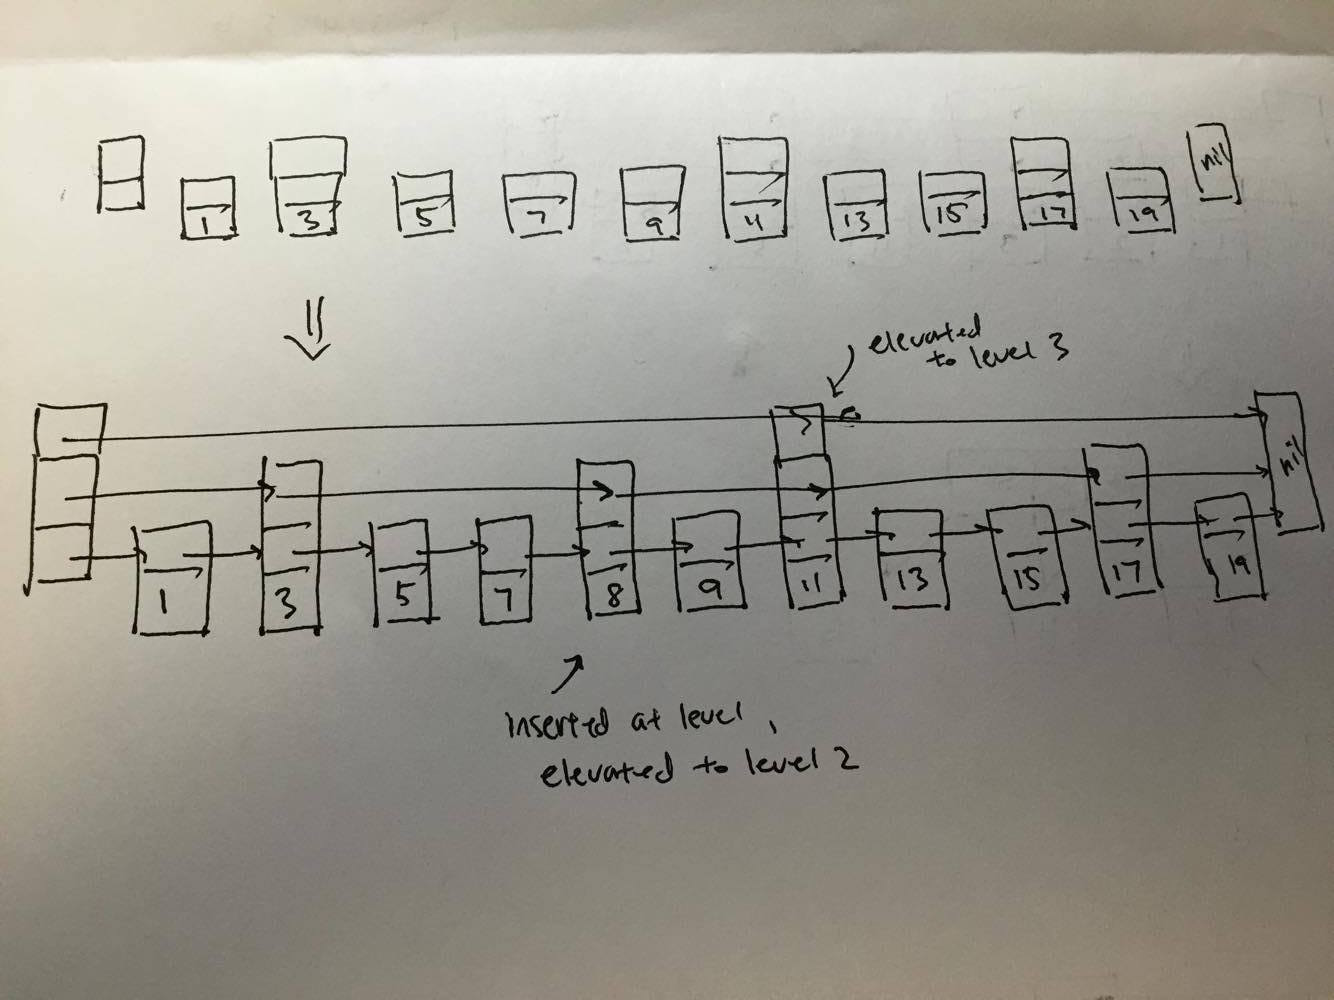
\includegraphics[scale=.3]{4iv}


  \end{enumerate}
\end{enumerate}

\end{document}



%%% Local Variables:
%%% mode: latex
%%% TeX-master: t
%%% End:
